\documentclass{beamer}

\usetheme{Madrid}

% Color settings
\setbeamercolor{normal text}{bg=white, fg=black}
\setbeamercolor{alerted text}{bg=white, fg=black}
\setbeamercolor{structure}{bg=white, fg=cyan!70}
%\setbeamercolor{navigation symbols}{bg=white, fg=white}
\setbeamercolor{title}{bg=cyan!7, fg=black}
\setbeamercolor{subtitle}{bg=white, fg=black}
\setbeamercolor{section in toc}{bg=white, fg=black}
\setbeamercolor{subsection in toc}{bg=white, fg=black}
\setbeamercolor{frametitle}{bg=cyan!7, fg=black}
\setbeamercolor{block title}{bg=white, fg=black}
\setbeamercolor{block title alerted}{bg=white, fg=black}
\setbeamercolor{block title example}{bg=white, fg=black}
\setbeamercolor{section number projected}{bg=white, fg=black}

% Header/Footer colors
\setbeamercolor{author in head/foot}{bg=cyan!7,fg=black} 
\setbeamercolor{title in head/foot}{bg=cyan!7,fg=black} 
\setbeamercolor{date in head/foot}{bg=cyan!7,fg=black} 
\setbeamercolor{page number in head/foot}{bg=cyan!7,fg=black}

% Redefine section in toc to include section numbers
\setbeamertemplate{section in toc}{\inserttocsectionnumber.~\inserttocsection}
\setbeamertemplate{navigation symbols}{}
%\setbeamertemplate{frametitle}[default][center]

\usepackage{graphicx} % for including graphics
\usepackage{multicol}

\title[Construction Union\ldots{Historical-Comparative}]{Construction Union Agreements\\
Union Organizing in Historical-Comparative Perspective}
\author{Matthew Carson}
\date[Undergrad. Research Week '24]{Undergraduate Research Week 2024}

\begin{document}

\begin{frame}
  \titlepage
\end{frame}

\begin{frame}{Table of Contents}
  \begin{multicols}{2}
    \tableofcontents
  \end{multicols}
\end{frame}

\section{Introduction}
\begin{frame}{Introduction}
	US Building Trade unions organize their workers differently. Most labor unions compel employers to negotiate, but the Building Trades engage in voluntary negotiations, relying on workers' skill levels rather than strike leverage. 
	\newline\newline
	\textbf{Building Trades (BT)}
	\begin{itemize}
		\item Are frequently political outliers.
		\item Oppose progressive environmental policies.
		\begin{itemize}
			\item Alignin more closely with the petrochemical industry (e.g., pipelines).
		\end{itemize}
		\item Are not supportive of single-payer healthcare.
	\end{itemize}

\textbf{Do the ways that unions organize affect their political stances and how solidaristic they are with progressive movements?}
	
	%This approach correlates with their frequent political deviations from the broader US labor movement, particularly in opposing progressive environmental policies and aligning more closely with the petrochemical industry on environmental issues, and not supporting single-payer healthcare.
\end{frame}

\section{Methods}
\subsection{Historical}
\begin{frame}{Methods:Historical}
\setlength{\arrayrulewidth}{0.0pt} % Set the thickness of the rules to 0
\begin{tabular}{|p{0.3\textwidth}|p{0.6\textwidth}|}
\hline
\begin{minipage}[t][0.2\textheight][t]{\linewidth}
\textbf{Historical\\
Within-Case\\
Analyses}
\end{minipage}
&
\begin{itemize}
    \item Historical trajectory of the union.
    \item Durability: institutional arrangements.
    \item Structural features \& constraints.
    \item Institutional changes (mergers, etc.).
    \item Evolutionary or generative approach. %\footnote{Reed 1997}
\end{itemize}
\\
\hline
\begin{minipage}[c][0.2\textheight][b]{\linewidth}
\textbf{Comparative\\
Between-Case\\
Analyses}
\end{minipage}
&
\begin{itemize}
    \item Differences in institutional features.
    \item Difference in political outcomes.
\end{itemize}
\\
\hline
\end{tabular}
\end{frame}

\subsection{Interviews}
\begin{frame}{Methods: Interviews}
\begin{itemize}
	\item While the Building Trades largely ``organizes the bosses" rather than the workers already employed, there is still some variation in how they organize. 
	\item National Labor Relations representation case petition database
	\begin{itemize}
		\item 98 building trades unions filed for a representation election in 2023.
	\end{itemize}		 
	\item Emails were sent to union's office or organizer (email addresses from the union's website.)
	\item Three union organizers were interviewed.
\end{itemize}
\end{frame}

\section{Cases}
\begin{frame}{Case Selection}
	\begin{itemize}
		\item \textbf{Historical}
		\begin{itemize}
			\item United Association of Plumbers and Pipefitters Local 189
			\item Oil Chemical and Atomic Workers Union (now part of the United Steelworkers)
			\item International Association of Machinists
		\end{itemize}
		\item \textbf{Interviews}
		\begin{itemize}
			\item Millwrights
			\item Electricians
			\item Operative Plasterers \& Cement Masons
		\end{itemize}
	\end{itemize}
\end{frame}

\section{Union Organizing Paths}
\subsection{NLRB Election}
\begin{frame}{Union Organizing Paths: NLRB Election}
  \begin{columns}
    \column{0.725\textwidth}
    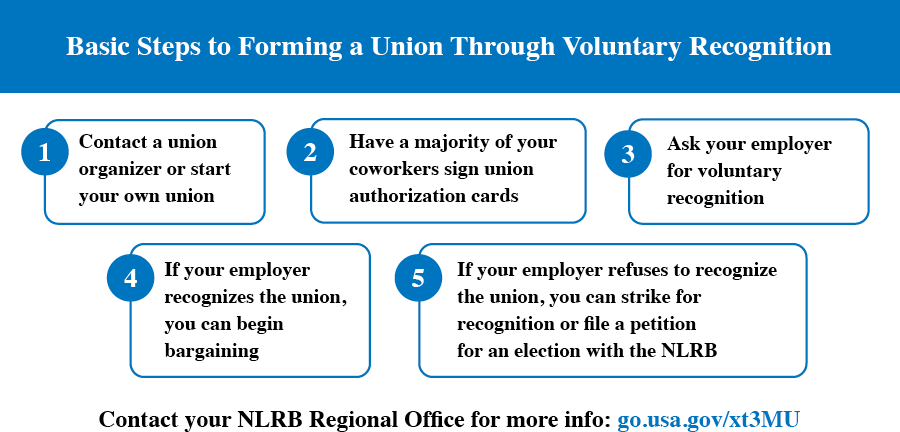
\includegraphics[width=0.9\linewidth]{../images/DOL}
    \begin{scriptsize}
	    \begin{center}
	    	(Source: US Department of Labor.)
	    \end{center}    
    \end{scriptsize}
    
    
    \column{0.275\textwidth}
     Designed for the \underline{industrial unions} forming at the time of the passage of the National Labor Relations Act.
    \newline\newline
    However, it was not designed for the Building Trades because they were already organizing differently.

    \end{columns}
\end{frame}

\subsection{Comparison}
\begin{frame}{Union Organizing Paths: Comparison}
  \begin{columns}
    \column{0.725\textwidth}
    \includegraphics[width=0.9\linewidth]{../images/organizing_paths}

    \column{0.275\textwidth}
    The industrial mode of organizing (left) and the construction mode of organizing (right).\newline\newline
    Construction unions may follow either path, but other unions may not voluntarily negotiate the way that construction unions can.
    \end{columns}
\end{frame}

\section{Building Trades Leverage}
\begin{frame}{Building Trades Leverage}
  \begin{columns}
    \column{0.725\textwidth}
    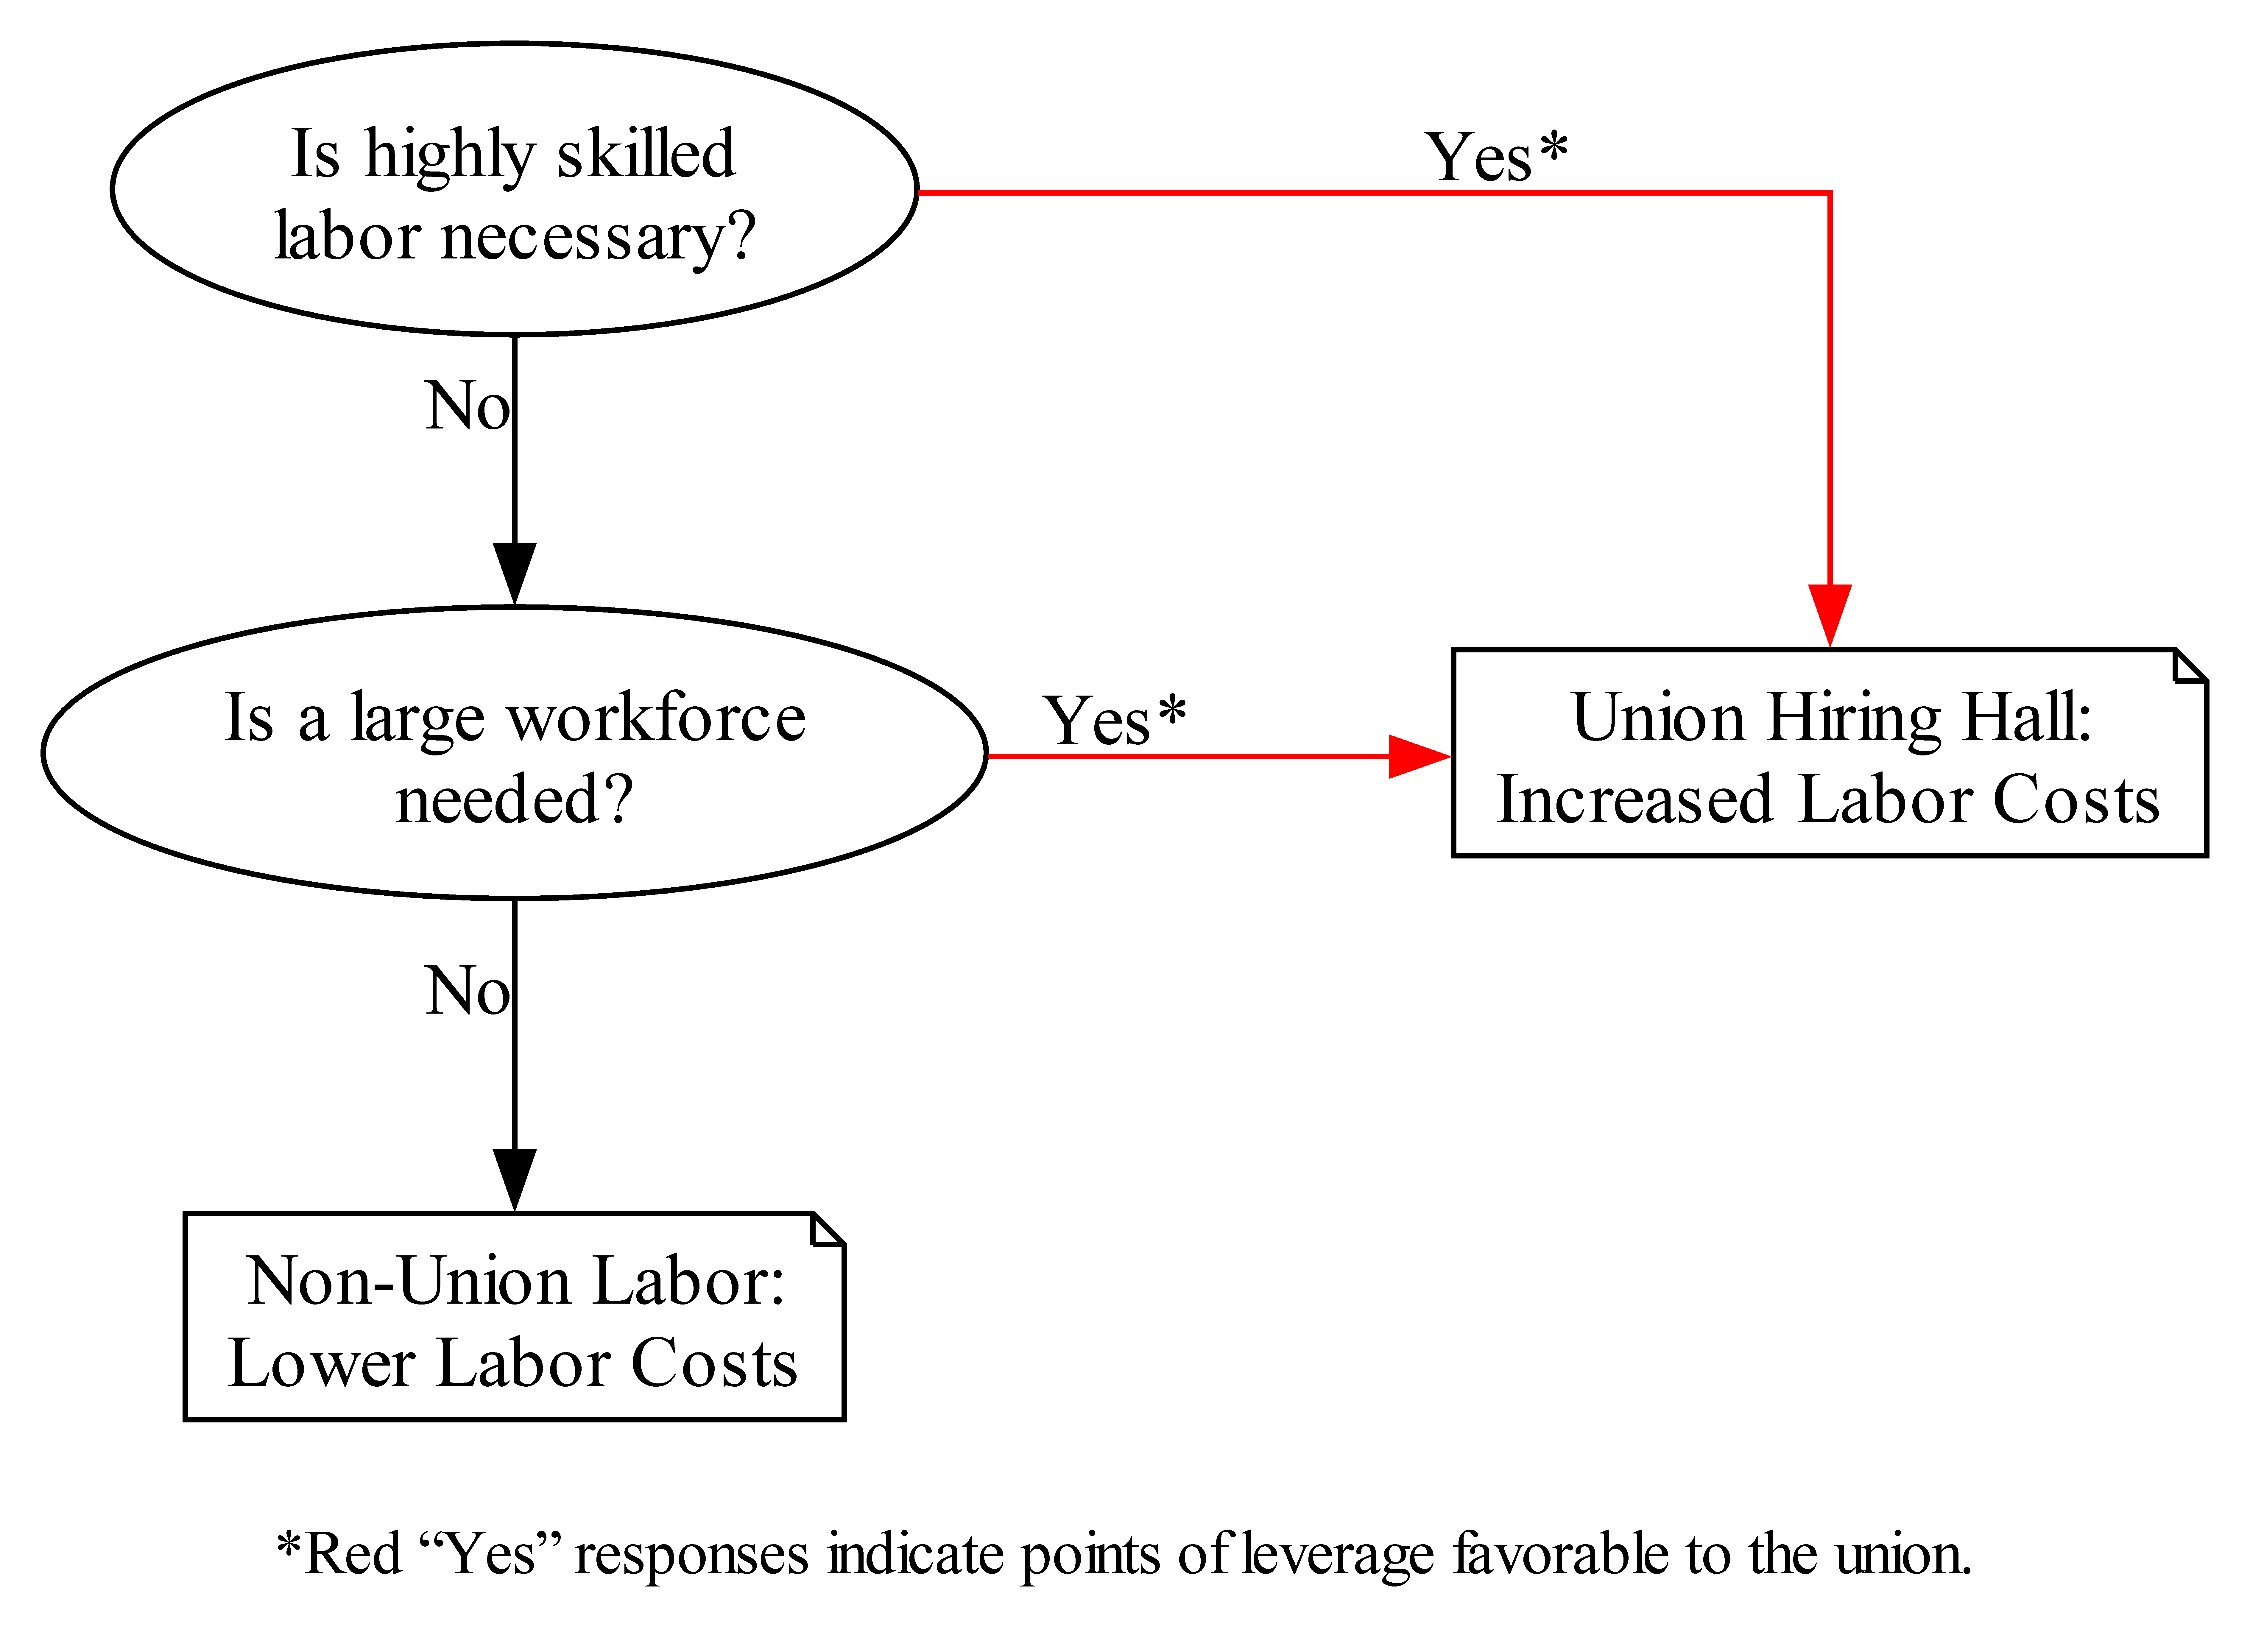
\includegraphics[width=\linewidth]{../images/union_power_red}

    \column{0.275\textwidth}
    Construction unions have more leverage where the employer requires a more skilled workforce or where the job is large and requires many employees.
  \end{columns}
\end{frame}

\section{Building Trades Hiring Hall}
\begin{frame}{Building Trades Hiring Hall}
	\begin{columns}
	\column{0.725\textwidth}
	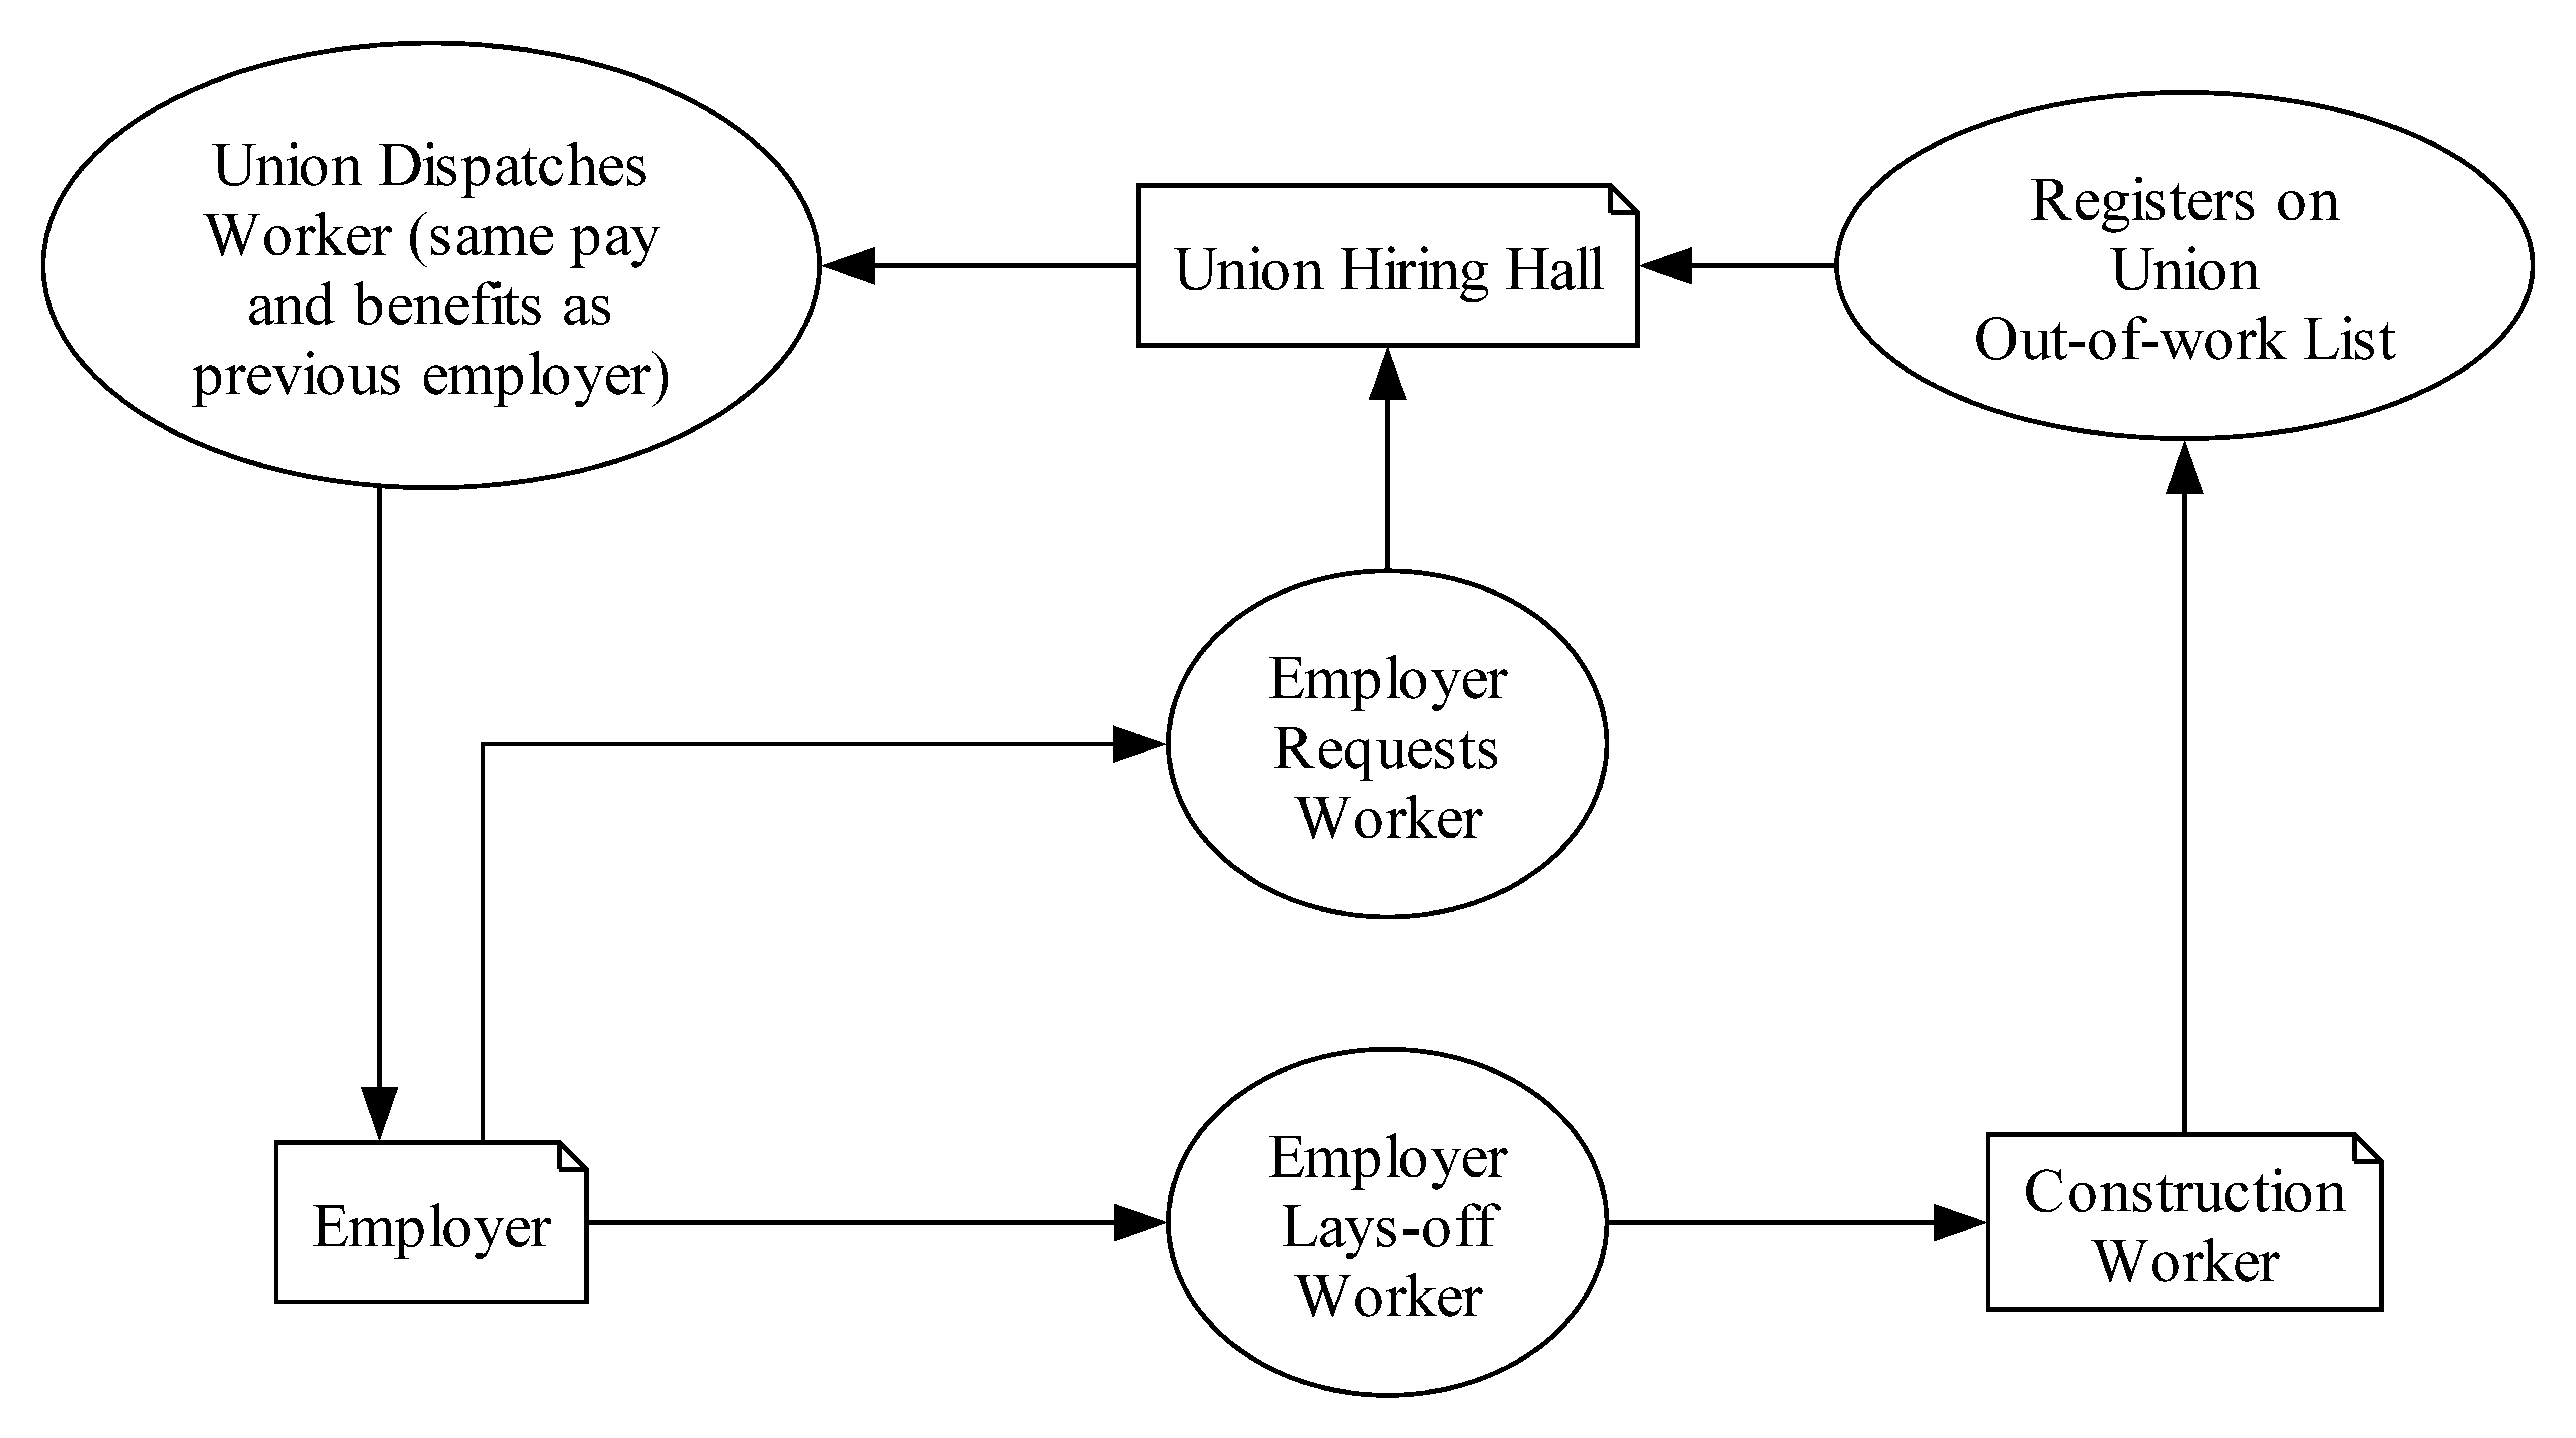
\includegraphics[width=\linewidth]{../images/hiring_hall}
	\column{0.275\textwidth}
	When employers require more workers for their projects, they contact the hiring hall to request workers to be dispatched to the job site.
	\end{columns}
\end{frame}

\section{OCAW/USW vs. UA}
\begin{frame}{OCAW/USW vs. UA}
\textbf{Do unions with petrochemical work tend to align themselves with the petrochemical industry?}\newline

This is \emph{not} necessarily the case.
	\begin{itemize}
		\item The UA and OCAW/USW have taken very different political stances regarding clean energy transition.
		\item OCAW/USW has embraced a ``Just Transition" from dirty to clean energy.
	\begin{itemize}
		\item ``Just Transition": workers affected by the closure of plants, refineries, etc. are offered a safety net while transitioning to another career.
	\end{itemize}
	\item The United Association (UA) of Plubmers and Pipefitters (Building Trades) supports petrochemical industry friendly policies.
	\end{itemize}
\end{frame}

\subsection{Institutional consolidation}
\begin{frame}{OCAW/USW vs. UA: Institutional consolidation}
	\begin{itemize}
		\item United Association (UA)		
			\begin{itemize}
				\item Apprenticeship and training as a ``bargaining chip."
				\item Prehire agreements are the norm.
				\item Institutional/structural features shaped the mode of organizing that the BT adopted.
				\begin{itemize}
					\item They could have chosen a different mode.
					\item They became a junior partner to capital because of how they chose to organize.
				\end{itemize}
	\end{itemize}
		\item OCAW/USW
		\begin{itemize}
			\item Never became a junior partner to capital — relationship antagonistic
		\end{itemize}
	\end{itemize}
\end{frame}





\subsection{Different occupational context}
\begin{frame}{OCAW/USW vs. UA: Different occupational context}
	\begin{itemize}
		\item United Association (UA)
		\begin{itemize}
			\item The pre-hire agreement made the movement between employers with the same wages/benefits possible.
			\item Hiring hall formed as an institution
		\end{itemize}
		\item OCAW/USW
			\begin{itemize}
				\item Same plant entire career
			\end{itemize}
	\end{itemize}
\end{frame}


\subsection{Political context}
\begin{frame}{OCAW/USW vs. UA: Political context}
	\begin{itemize}
		\item United Association (UA)
		\begin{itemize}
			\item Never had Communist Party or socialist connections
		\end{itemize}
		\item OCAW/USW
			\begin{itemize}
				\item Historically had Communist Party members
			\end{itemize}
	\end{itemize}
\end{frame}

\subsection{The Line Between Worker \& Owner}
\begin{frame}{OCAW/USW vs. UA: The Line Between Worker and Owner}
	\begin{itemize}
		\item United Association (UA)
		\begin{itemize}
			\item Construction firms are small
			\item Union members as worker-owners — infrequent, but it happens.
		\end{itemize}
		\item OCAW/USW
			\begin{itemize}
				\item Members are always wage workers.
				\item Employers are usually large multi-nationals
			\end{itemize}
	\end{itemize}
\end{frame}


\section{Machinists (IAM) vs. UA/Building Trades}
\begin{frame}{Findings: Machinists (IAM) vs. UA/Building Trades}
\textbf{Do craft unions that organize via the industrial path support more progressive policies?}\newline
	\begin{itemize}
		\item The Machinists (IAM), while in the AFL, faced challenges similar to those that the industrial unions faced.
		\item Example: IAM District Lodge 751
		\begin{itemize}
			\item Aerospace work at Boeing (essentially manufacturing).
			\item Highly skilled craft workers but organized via the industrial union path.
			\item No prehire agreements or hiring hall.
		\end{itemize}
	\end{itemize}
\end{frame}



\subsection{Inter-union conflicts}
\begin{frame}{Machinists (IAM) and Longshore Workers (ILWU): Inter-union conflicts}
	\begin{itemize}
		\item But the international union has maintained a craft union orientation like the building trades.
		\item Inter-union conflict with the Longshore Workers Union (ILWU).
		\begin{itemize}
			\item ``Union Turf Wars Expected to Heat Up"\footnote{\tiny Mongelluzzo, Bill. 2014. “Union Turf Wars Expected to Heat Up.” \textit{Journal of Commerce}, March 6.}
			\item Jurisdictional disputes between Longshore Union (ILWU) and Machinists (IAM) at ports along the West Coast.
		\end{itemize}
	\item Still, the international union supports progressive policies.
		\begin{itemize}
			\item Listed as a supporter at Labor for Single-Payer Healthcare.
			\item No Building Trades union is listed as a supporter.
		\end{itemize}
	\end{itemize}
\end{frame}
	


% Findings: Intra-Building Trades
\section{Intra-Building Trades}

\begin{frame}{Intra-Building Trades: Interviews}
\textbf{Do Building Trades unions that organize using the industrial path show more solidarity with community groups or other unions? Do they support more progressive political policies?}\newline
	\begin{itemize}
%		\item I expected to find building trades (BT) unions that organize this way to be more involved in community and progressive organizations and other labor organizations.
		\item By and large, this is \emph{not} the case.
		\item They pursue this strategy for pragmatic reasons.
		\begin{itemize}
			\item Not indicative of a different political orientation.
		\end{itemize}
		\item BT unions pursue different organizing strategies depending on the conditions.
		\item BT unions often use this approach for service-based employers or where employers have a permanent workforce — usually not construction work.
		\item No “spillover” into the construction side of the union.
	\end{itemize}
\end{frame}



%\section{Conclusion}
%\begin{frame}{Conclusion}
%  \begin{itemize}
%  	\item The Building Trades 
%  \end{itemize}
%\end{frame}

\end{document}
